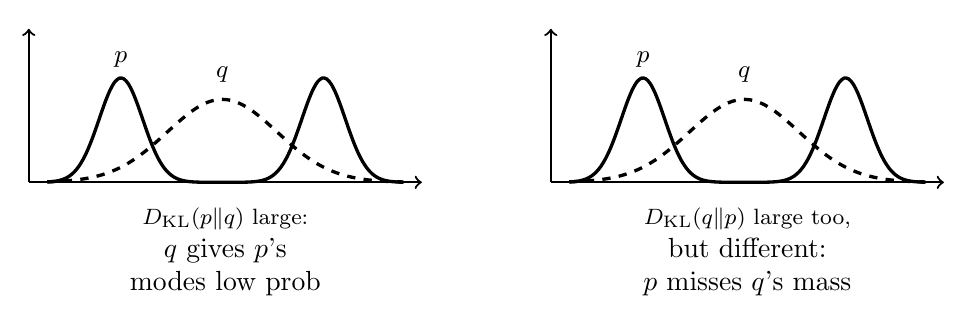
\begin{tikzpicture}[scale=0.78]
% two small multiples: target p bimodal; q single central bump
\foreach \cx/\captext in {0/{$D_{\mathrm{KL}}(p\|q)$ large:\\ $q$ gives $p$'s\\ modes low prob}, 8.5/{$D_{\mathrm{KL}}(q\|p)$ large too,\\ but different:\\ $p$ misses $q$'s mass}}{
  \begin{scope}[xshift=\cx cm]
    \draw[->, thick] (0,0) -- (6.4,0);
    \draw[->, thick] (0,0) -- (0,2.5);
    % p: bimodal
    \draw[very thick, domain=0.3:6.1, smooth, samples=80]
      plot (\x, {1.7*exp(-((\x-1.5)^2)/0.25) + 1.7*exp(-((\x-4.8)^2)/0.25)});
    \node[font=\small] at (1.5,2.0) {$p$};
    % q: single center bump
    \draw[very thick, dashed, domain=0.3:6.1, smooth, samples=80]
      plot (\x, {1.35*exp(-((\x-3.15)^2)/1.6)});
    \node[font=\small] at (3.15,1.75) {$q$};
    \node[align=center, below] at (3.2,-0.25) {\footnotesize\captext};
  \end{scope}
}
\end{tikzpicture}
